%!tex root = ../report.tex

\section{Quality of Service}
Quality of service are performance guarantees given to customers in a service level agreement (SLA).
These performance guarantees might be important for different scenarios like streaming, interactive applications (games,\dots) or safety-critical application or safety-critical applications.
SLAs are applied at different levels: packet, flow, application or user level.
To guarantee the specifications in an SLA one has to perform different tasks:
\begin{itemize}
  \item Modelling: Understand which parts of the network have an impact on the SLA\\
    These usually are propagation, processing, transmission and queuing delay.
  \item Classification: Identify which packet need SLA\\
    Several methods exist for identification like using packet header fields like IP-5-Tuple or IPv4 TOS field or another alternative is to do deep packet inspection.
  \item Scheduling: Give preferential service to network packets.
    Two types of schedulers can be differentiated: work-conserving schedulers only are idle if no packet available whereas non-work conserving ones might be idle even if packets are pending.\\
    The common architecture for scheduling is to have multiple queues with different priorities.
    The queues are pulled if all queues with higher priority are empty.\\
    A slight deviation of this approach is round robin, where the queues are polled after one another.\\
    A third approach namely \textbf{weighted fair queuing} tries to solve the problem of round robin queueing, where the bandwidth per queue depends on the packet sizes, and priority queue scheduling (starvation) by splitting the actual available bandwidth according to the weights of different queues.
    The implementation is much more complex though and thus it is rarely used in real switches.
  \item Monitoring: Check actively or passively if SLAs are met\\
    This can be done with live tests, emulations or simulations or formal verification methods.
    The more critical real-time requirements an application has, the more precise the measuring algorithms typically are.
\end{itemize}

\subsection{Deterministic Network Calculus}
Network calculus is a framework developed for analyzing performance guarantees in networks of queues and schedulers.
In the deterministic variant, no randomness is involved whereas the stochastic model includes randomness and thus is characterized in probabilistic terms.\\
Packets and network protocols are described as \textbf{flow}, meaning an unidirectional set of packets going from a sender to a receiver and are modeled by a \textbf{cumulative arrival function} A.
$A(t)$ represents the amount of data sent by the flow in the time interval $[0,t)$.The 
The \textbf{deterministic arrival curve} then is defined as $A(t) - A(s) \leq \alpha (t-s), \forall 0 \leq s \leq t$.
A simple example for this would be the \textbf{token bucket} $y_{r,b}(t,s) = r \cdot (t-s) + b$ where r denotes the average rate and b the burstiness parameter.\\
Queues and schedulers are seen as \textbf{servers} in network calculus.
They have a \textbf{deterministic service curve $\beta$} such that the output curve $A^* \geq \inf_{0 \leq s \leq t} \{A(s) + \beta (t-s)\}$
A simple example for this is the \textbf{rate-latency} which is defined as $\beta_{R<T}(t) = R[t - T]^+$ where R is the rate, T the processing delay and $[x]^+ = max(0,x)$.\\
Delay is defined as time time it takes for a packet to traverse the queue and queue size as the backlog size at the server.
For a visualization see Figure~\ref{fig:nc_delay_and_backlog}.
\begin{figure}[h]
  \centering
  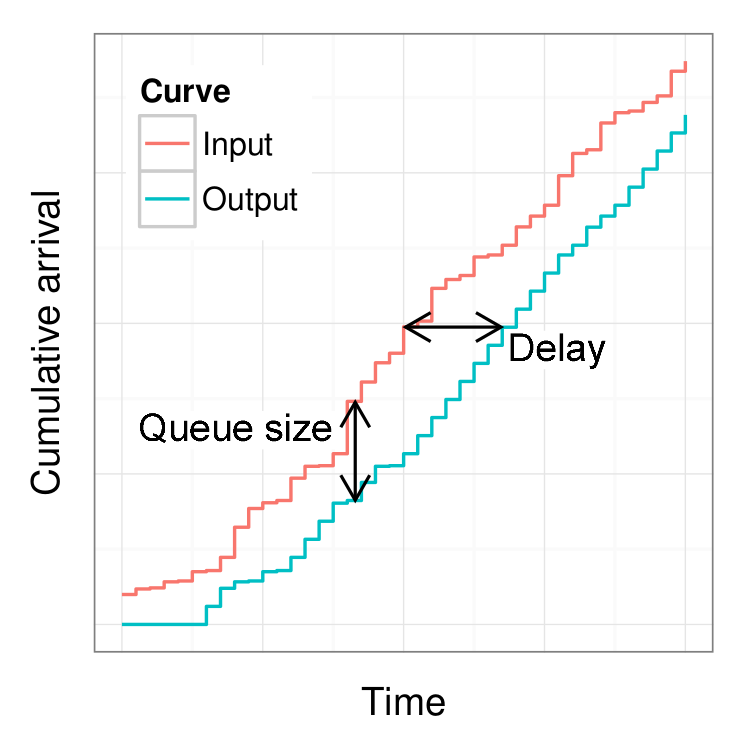
\includegraphics[width=.4\textwidth]{figures/nc_delay_and_backlog.png}
  \caption{Delay and Backlog}\label{fig:nc_delay_and_backlog}
\end{figure}

Deterministic network calculus can be used when there are no cyclic dependencies, no feedback loops, no simple analysis exists (state explosion) and when a good model of the traffic is known.

\subsection{Stochastic Network Calculus}
In stochastic network calculus flows are defined by a sequence of non-negative, real random variables $(a_n)_{n \in \mathds{N}}$ of random size.
Their cumulative arrival up to time n is then defined as $A(n) = \sum^n_{i=a}a_i$.
$(a_n)$ can follow any random distribution and are considered to be independent and identically distributed.
Similar to DNC, service curves are $S(n,m)$ of a server are defined as $A^*(n) \geq \inf_{0 \geq k \geq n} \{A(k) + S(k,n)\}$ where $S(n,m)$ can either be a stochastic or deterministic process.\\

Stochastic network calculus is mainly used for video streaming, protocols with feedback loops, wireless networks or energy networks.

\subsection{QoS in IP Networks}
In modern IP networks traffic is usually limited to a fixed set of declared parameters concerning average, peak rate and burst size.
To implement these limits, a token bucket can be used which fills with a pre-specified rate until it is full.
The limitation is then given by the cost of forwarding of one token.
To guarantee an upper bound, this approach can be combined with WFQ.

\subsubsection*{IETF Integrated Services}
The IETF integrated services provide an architecture for providing QoS guarantees in IP networks for individual application sessions.\\
If a flow/call arrives, resources have to be requested with information about the estimated traffic and reservation characteristics.
Routers then decide based on this information and remaining unreserved resources if the request can be accepted and answers accordingly.\\
Two service models are possible here.
A guaranteed service where worst-case traffic is important or a controlled load service where the QoS closely corresponds to the QoS that the same flow would receive from an unloaded network.

\subsubsection*{IEFT Differentiated Services}
IEFT Differentiated Services want qualitative service classes (platinum, gold, silver services).
Implementation here differs regarding core and edge nodes.
The edge routers look at the per-flow traffic, marks packets according to a class as "in-profile" or "out-profile" and forwards to core nodes regarding a token bucket.
The core nodes then only look at the packet classes and do buffering and scheduling according to that information where "in-profile" packets have higher priority.

\subsubsection*{Classification and Conditioning}
For classification the TOS field of the IPv4 header or the Traffic class field of the IPv6 header can be used.
They consist 2 bits for a explicit congestion notification (ECN) and 6 bits that can be used for Differentiated Service Code Point (DSCP) and per hop behaviors (PHB).\\
Developed PHBs:
\begin{itemize}
  \item Expedited Forwarding: logical link with a minimum guaranteed rate.
  \item Assured Forwarding: 4 classes of bandwidth with defined guaranteed minimum bandwidth and buffering, packets can have one of three possible drop preferences
\end{itemize}

\subsection{Resource Reservation Protocol (RSVP)}
RSVP is used to communicate/signal requirements to the network.
This is done by sending information about the QoS that is required (r-spec) and the characteristics of the traffic that will be sent into the network (t-spec) to routers.\\
More precisely senders and receivers first join a multicast group.
The sender then sends a path message to make its presence known to the routers which store path states which consist of the IP address of the previous node and a sender template (data format of the sender), sender t-spec and adspec (advertisement data).
In the end a path teardown message is sent to remove the path state from routers.\\
The receiver send a reservation message to reserve resources from sender(s) to receiver.
At every node, the destination IP changes to the next node on the reverse path and the source IP gets the address of the previous node.
In the end a reservation teardown message is sent to remove reservations.
The network only sends messages when errors occur.

\subsection{Maintaining Network State}
A state in this context is defined as information stored in network nodes by network protocols.\\
A \textbf{hard state} is installed on receiving a setup message from the sender and only removed when getting a teardown message or sometimes a heartbeat is used.
A \textbf{soft state} on the other hand is also created when receiving a setup or trigger message from the sender but is removed when the connection times out. 
For this reason a heartbeat is definitely necessary.\\
Senders in this context are nodes that (re)generate signaling messages to install, keep and remove states.
Receivers on the other hand are nodes that creates, maintains and removes states based on the messages of the sender.\\

The advantage of soft state over hard state here is that no explicit error messages need to be sent to indicate problems.
In case of a failed link the update messages will update the routes and in case of a failed host the connection will just time out.
A problem is though that if the first path message gets lost the timeout might be quite long to retry.
For that reason ACK messages can be used from receiver to sender to be able to use a quicker timeout than the normal heartbeat.
